%%%----------------------------------------------------------
\chapter{Correlation-Based Subimage Matching}
%%%----------------------------------------------------------

The task of this assignment to locate matches to a selected region of interest in an image. We do not only want to find the perfect match we want to find all possible matches by calculating a distance map for every possible position in the image. This map should give information about all possible match positions. To calculate this map three different methods are used: \textit{Sum of Squared Distances}, \textit{Linear Cross Correlation} and the \textit{Normalized Cross Correlation}. The matches are selected by calculating local minima and maxima.

\section{Algorithm}
To find potential matches for the reference image $R$. $R$ is moved across the image $I$ and for each position a difference value between $R$ and the current position of $I$ is calculated using a \textit{scoring function}. These difference values are stored at their respective positions in the distance map. The following steps were performed the accomplish the desired outcome:
\begin{enumerate}
	\item Select a region of interest in the image $I$ which will be the mentioned reference image $R$.
	\item The slide $R$ across $I$ and create the distance as discussed. Keep in mind that the reference image must always be inside the boundaries of $I$. This means the sliding starts at (0,0)but has to end at ($I_w - R_w, I_h - R_h$).
	\item Calculate the distance map using one of the three scoring functions.
	\item Look for local maxima/minima in the distance map to find the best matches.
\end{enumerate}

\subsection{Scoring functions}

As mentioned in the beginning there are three different scoring functions used to create the distance map:
\begin{itemize}
	\item Sum of Squared Distances
	\begin{equation}
		D(r,s) = \left[ \sum_{(i,j) \in \R} \vert I(r+i,s + j) - R(i,j)\vert^2\right]^{\frac{1}{2}}
	\end{equation}
	\item Linear Cross Correlation
	\begin{equation}
		D(r,s) = \sum_{(i,j) \in \R} I(r+i,s + j) \cdot R(i,j)
	\end{equation}
	\item Normalized Cross Correlation
	\begin{equation}
		D(r,s) = \frac{\sum_{(i,j) \in \R} I(r + i,s +j) \cdot R(i,j)}{\left[\sum_{(i,j) \in \R} I^2(r+i,s+j)\right]^{\frac{1}{2}} \cdot \left[\sum_{(i,j) \in \R} R^2(i,j)\right]^{\frac{1}{2}}}
	\end{equation}
\end{itemize}

\subsection{Finding local maxima/minima}
Too find local maxima i took a rather basic approach. I compared each value with the value of all their neighbors. If all the neighboring values in the distance map had a lower/higher value a local maxima/minima was found. All found maxima/minima are added to a list.

\section{Results}
The Sum of Squared Distances scoring function delivered the best results. It was able to successfully find the the sphinx in the test image (see figure \ref{fig:8_1} and \ref{fig:8_2}). The normalized cross correlation led to a similar result but with a worse distance difference at non-matching positions. The linear cross correlation was less reliable and highly varied between test images and it was strongly influenced by bright spots on the image. It did not find the sphinx successfully and marked the sky instead (figure \ref{fig:8_3}, and \ref{fig:8_4}).

When trying to match repetitive patterns the linear cross correlation was again not able to detect the patterns. The sum of squared distances as well as normalized cross correlation delivered acceptable results and were able to detect most of the bomb craters in the test image \textit{bomb-craters-3} (figure \ref{fig:8_5}). The normalized cross correlation was also more robust and allowed higher tolerance values.

\begin{figure}
	\centering
	\begin{minipage}[t]{0.49\linewidth}
		\centering
		\frame{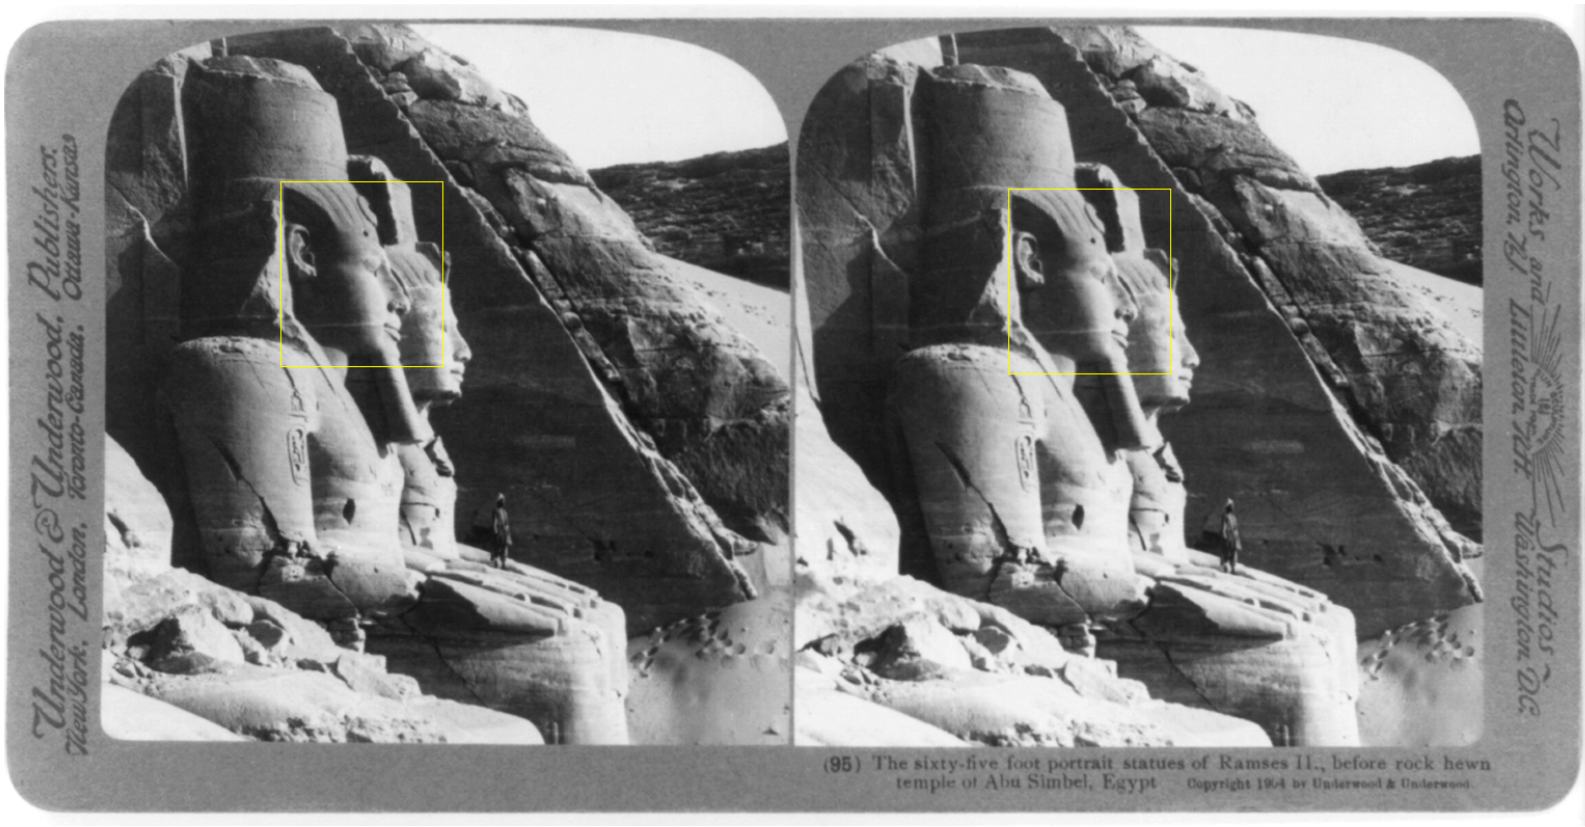
\includegraphics[width=.98\linewidth]{images/ssd_image}}
		\caption{The detected region of interest in the sphinx test image with the Sum of Squared Distances.}
		\label{fig:8_1}
	\end{minipage}
	\hfill
	\begin{minipage}[t]{0.49\linewidth}
		\centering
		\frame{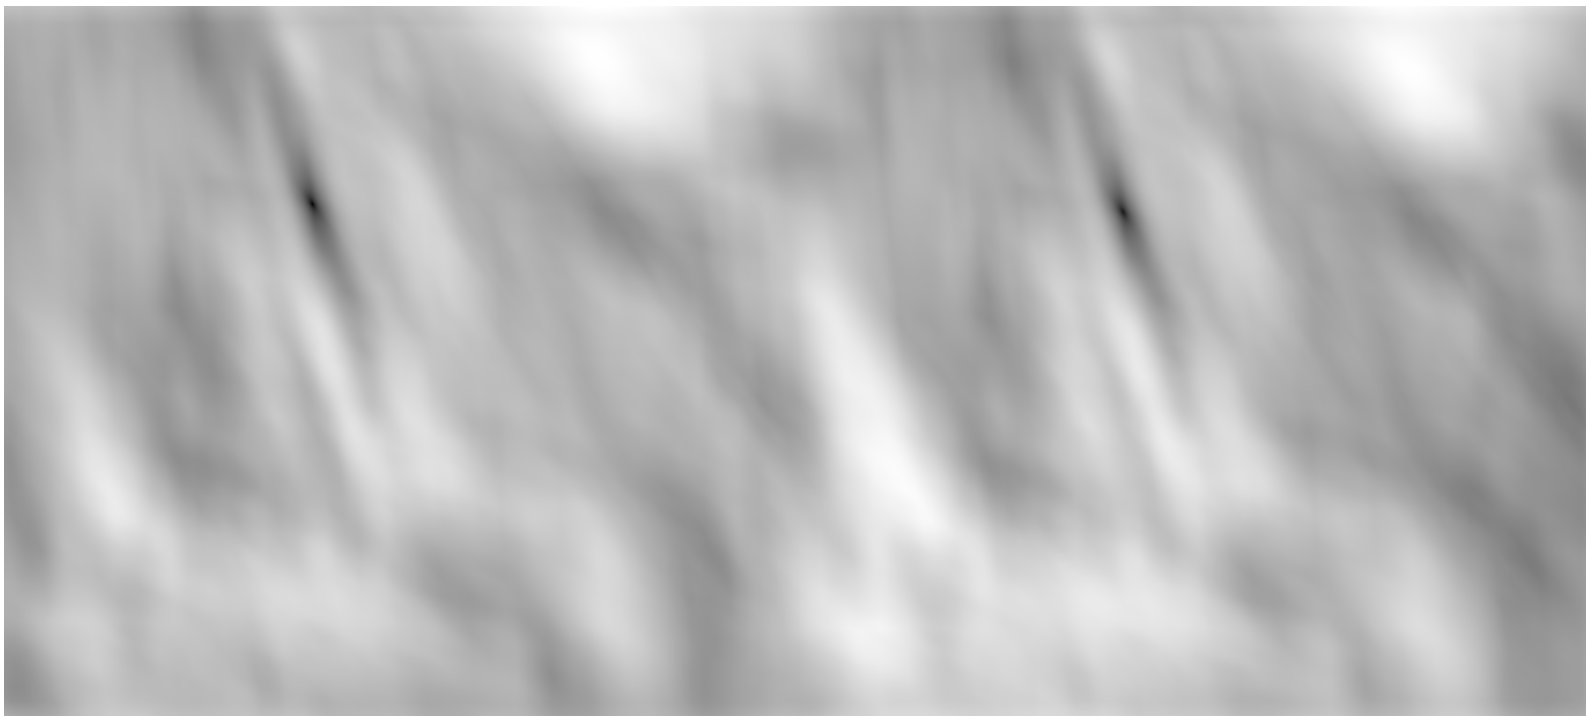
\includegraphics[width=.98\linewidth]{images/ssd_distance}}
		\caption{The distance map using the Sum of Squared Distances on the sphinx test image.}
		\label{fig:8_2}
	\end{minipage}
\end{figure}

\begin{figure}
	\centering
	\begin{minipage}[t]{0.49\linewidth}
		\centering
		\frame{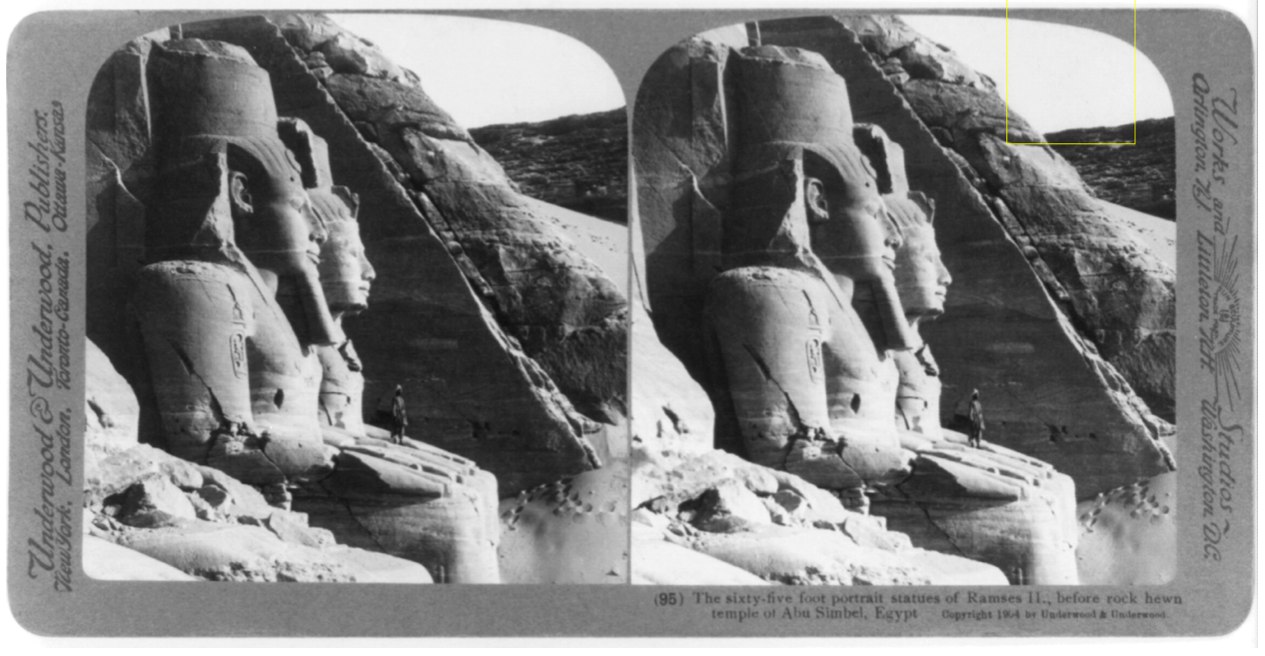
\includegraphics[width=.98\linewidth]{images/lcc_image}}
		\caption{The detected region of interest in the sphinx test image with linear cross correlation.}
		\label{fig:8_3}
	\end{minipage}
	\hfill
	\begin{minipage}[t]{0.49\linewidth}
		\centering
		\frame{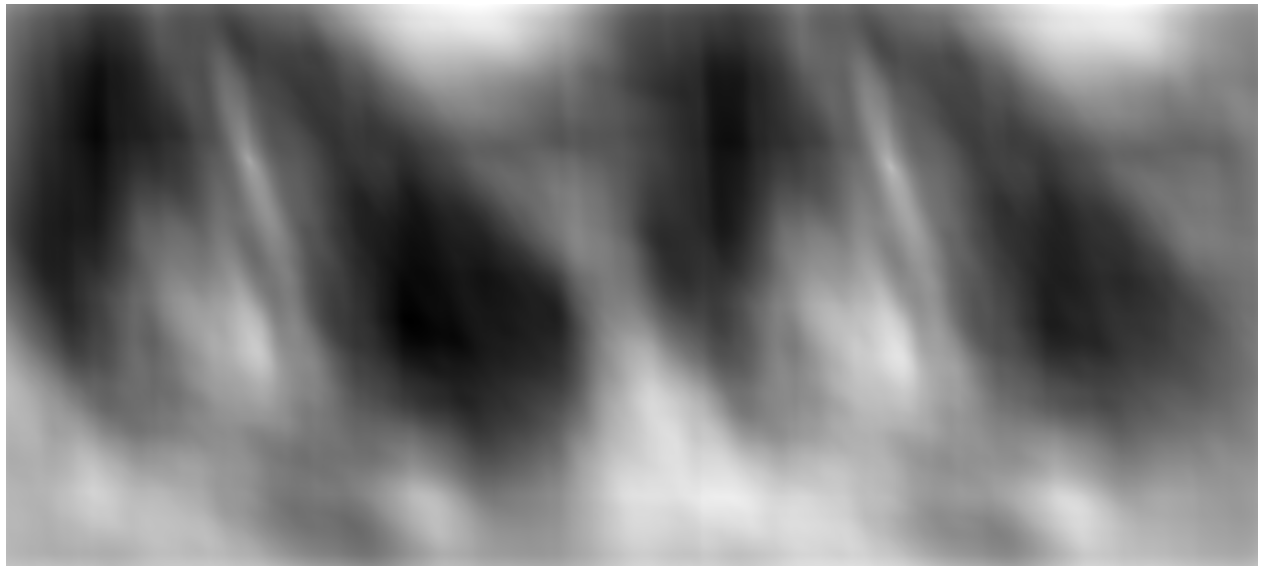
\includegraphics[width=.98\linewidth]{images/lcc_distance}}
		\caption{The distance map using linear cross correlation on the sphinx test image.}
		\label{fig:8_4}
	\end{minipage}
\end{figure}

\begin{figure}
	\centering
	\frame{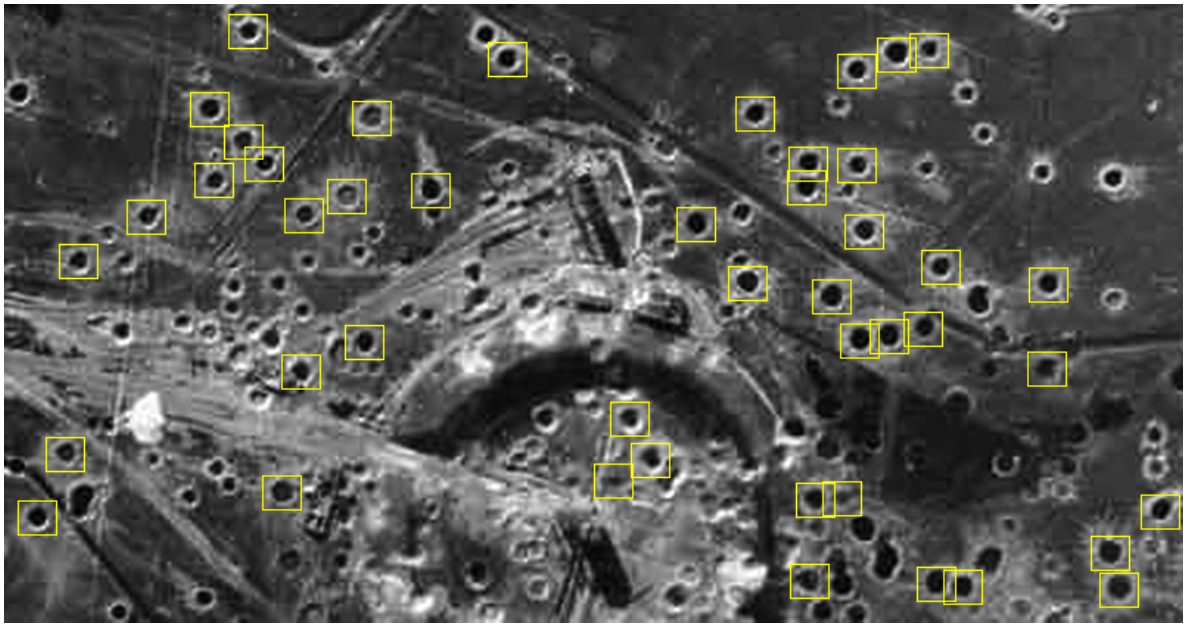
\includegraphics[width=0.9\linewidth]{images/ssd_rep}}
	\caption{The detected bomb craters using the Sum of Squared Distances and a tolerance value of 80\%.}
	\label{fig:8_5}
\end{figure}